% !TEX root = ../main.tex

\section{Results}

Our grounded theory analysis of industry documents resulted in the creation of 25 technical primitives, 18 technical properties, 11 normative properties, 11 capabilities, and 19 use case categories.
The technical primitives, technical properties, normative properties, and capabilities are shown in Figure~\ref{fig:grounded-theory-main} and the use case categories are shown in Figure~\ref{fig:grounded-theory-apps}.
In both Figures, the various items are connected with directional arrows; these arrows roughly represent a dependency relationship with the item being pointed to relying on the item that is being pointed from, though in most cases it is the relationship rather than the directionality of the arrow that is most important.

In this section, we describe how our results provide answers to three of our questions:  (1) what exactly is Blockchain technology, (2) what capabilities does it provide, (3) how does it compare to other approaches (e.g., distributed databases).

\subsection{What is Blockchain Technology?}
Our description of Blockchain technology is based on the technical primitives and properties identified during our analysis.
This analysis revealed three key components to Blockchain technology: shared governance and operation, a cryptographically-authenticated append-only ledger, and replication.
By themselves, these components are nothing new, but used together they form what is known as Blockchain technology or Blockchain for short.

\subsubsection{Shared Governance and Operation}
At the heart of Blockchain technology is the principle of shared governance and operation.
Either of these properties is common by itself; for example, having multiple parties govern how a system should function, but then relying up trusted-third parties to operate and maintain the system.
Alternatively, the literature is rife with well-defined systems that don't need ongoing governance, but require multiple parties to actually operate and maintain the system.

Blockchain is distinct, though, not necessarily unique, in that it requires a core set of participants---referred to hereafter as \emph{miners}---who are responsible for both deciding how the system should function (i.e., shared governance) and then for operating that system.
This type of shared governance is appropriate when miners are not able to sufficiently trust each other or a third-party to faithfully govern and operate a system.
By participating in all aspects of governance and operation, each miner can be assured that the system is operating as intended.
Even if one miner is compromised, the other miners retain the ability to detect malicious actions by the compromised miner and to prevent it from affecting the system.
In this regard, Blockchain technology provides \emph{diffused trust} wherein it is not individual miners that are not trusted, but rather the collective of all miners that is trusted.\footnote{This property has incorrectly been called ``trustlessness''. This is incorrect as trust still exists, it has just been diffused amongst multiple parties.} 

This shared governance and operation is executed using one or more \emph{consensus protocols} (e.g., proof-of-work~\cite{DN93,back1997partial,NakamotoS8}, byzantine fault tolerance~\cite{castro1999practical}).
The first consensus protocol is used by miners to determine what operations---known as \emph{transactions}---will be allowed to alter the state of the Blockchain system.
The second consensus protocol is used by miners to determine the rules that will be used to validate transactions in the first consensus protocol.
While governance could be conducted and recorded in transactions, removing the need for the second consensus protocol, we are not aware of any Blockchain systems that do so.

In practice, this second consensus protocol is usually an informal process in which changes to the first consensus protocol are discussed in a secondary channel (e.g., on an Internet discussion board), and consensus is established based on the number of miners that adopt the modified rules.
This ad-hoc consensus mechanisms means that it is possible for a Blockchain system to split, with one system being run by the set of miners continuing to operate using the original rules, and the other system being run by set of miners using the new rules.
Such a split is known as a \emph{fork}.
Often these forks are temporary, with miners either choosing to all adopt the new rules or to return to the original rules, but it is possible for a fork to result in the permanent creation of two non-interoperable Blockchain systems (e.g., Bitcoin Classic and Bitcoin Cash).

In Blockchain systems that use a majority-voting consensus mechanism for transaction validation, there is a concept of soft- and hard-forks.
In a soft fork, transactions that validate with the modified rules will also validate with the original rules, but transactions that validate with the original rules might not validate with the modified rules.
In a hard fork, transactions that validate with the modified rules will not necessarily validate with the original rules.
The benefit of a soft fork is that both sets of miners can continue participating in the first consensus protocol, with transactions following the modified rules always being accepted and the transactions following the original rules only being accepted if their is a majority of miners who still use the original rules.
While a soft-fork is not a permanent situation, it can provide time for miners to slowly adopt the modified protocol while allowing both sets of miners to operating on the same data.

Blockchain systems can be separated based on how they select who can act as miner:

\begin{itemize}
	\item \emph{Open governance.}
	Any party that is willing to participate in the consensus protocol is allowed to do so.
	As such, these systems are susceptible to Sybil attacks and it is necessary for them to use consensus protocols that rely on miners  proving ownership of some resource rather than relying on the miner's identity.
	Proof-of-work (demonstrating ownership of computing resources) and proof-of-stake (demonstrating ownership of digital assets stored by the Blockchain system) are the most common methods~\cite{Bano17,garay2018consensus}.
	
	\item \emph{Consortium governance.}
	Only approved miners that can attest to their identity are allowed to participate in the consensus protocol.
	The initial set of approved miners is defined at system initialization.
	If membership in the group of miners remains static over the lifetime of the system it is known as a \emph{static consortium}.
	Alternatively, in an \emph{agile consortium} miners change over time, either based on the rules of the system (e.g., random selection) or through consensus by the existing miners.
	Because miners in a consortium have a known identity they can use Byzantine Fault Tolerant consensus protocols, which do not require the resource expenditure of the Sybil-resistant protocols used in open governance-based systems~\cite{Bano17,garay2018consensus}.		
\end{itemize}

For each type of governance, there is a need to incentivize correct participant behavior.
The first type of incentive is an \emph{intrinsic incentive}---i.e., miners maintain the system faithfully because they derive value from using ie.
Next, \emph{on-chain incentives} are when the Blockchain system provides direct benefits to miners for faithfully executing the system (e.g., minting currency and giving it to the miners).
Finally, \emph{off-chain incentives} are any incentive that is not managed by the Blockchain system---for example, contractual obligations or reputation.
Importantly, off-chain incentives only apply to consortium governance as they inherently rely on knowing the identity of the miners.

\subsubsection{Append-Only Ledger}
While a Blockchain system might store its current state for convenience and performance, this is not actually an required in Blockchain technology.
Instead, the key data structure in Blockchain technology is a cryptographically authenticated data structure~\cite{tamassia2003authenticated} that stores a history of all the transactions that have been approved by the miners.
This \emph{ledger} provides full system provenance and allows for miners or other outside parties to audit the system.
In Bitcoin, this ledger is colloquially referred to as the ``blockchain'', but we avoid that term as it unnecessarily confusing to try and discuss both Blockchain (big-B) technology and the blockchain (little-b) data structure.

The first item in the append-only ledger is known as the \emph{genesis block}.
The genesis block is responsible for identifying the initial parameters for the system.
Whenever a new transaction is approved by the miners, it will be added to the ledger and cryptographically linked to one or more preceding transactions (or the genesis block for the first transaction)~\cite{bayer1993improving,haber1990time,haber1997secure}---for example, by signing a combination of the latest transaction and a hash of the transactions it is linked to.
The resulting data structure can be either linear (e.g., Bitcoin's hash chain) or branching (e.g., Merkle tree, directed acyclic graph).
Regardless of the underlying structure it is critical that all transactions are strictly ordered and that this ordering never changes.

Transactions stored in the append-only ledger can contain any data allowed by the consensus protocol, but in practice transactions are usually concerned with \emph{tokens}.
Tokens represent a resource that is either on-chain (e.g., cryptocurrency, a document) or off-chain (e.g., a diamond, a file stored in the cloud) and are used to track that resource within the Blockchain system.
For off-chain assets, there needs to be the ability to \emph{staple} the on-chain token to the off-chain assets.
While there have been a variety of proposals for doing this (e.g., etching the token's Id onto the physical items), effective stapling remains an open research challenge.

Tokens can also represent and store executable functions known as \emph{smart contracts}.
Users can execute these scripts by providing appropriate inputs.
The script is then executed by the miners with the output of the script being written to the append-only ledger in a transaction.
The computational power of these scripts is determined is determined by the Blockchain's consensus rules.

Whether a user of a Blockchain system is able to create, update, or delete a token is based on permissions defined by the miners.
While these permissions could be tracked using traditional access control paradigms, most often they are regulated cryptographically.
In this paradigm, when a token is created it is also associated with a public key.
The ability to update or delete this token is then granted to any users that can solve some cryptographic puzzle that would only be solvable with knowledge of the private key (e.g., generating a signature that validates with the public key attached to the token).
Ownership of the token can be transfered or shared by associating it with a new public key.

The biggest challenge towards key-based ownership of tokens is the need to manage a public key infrastructure (PKI).
This is both a hassle technically~\cite{CT} as well as for users~\cite{ruoti2015johnny,barber2012bitter}.
One advantage of having key-based, not user-based ownership of tokens is that allows for anonymity in the ownership and use of tokens.
Still, this requires careful attention in the system design to use appropriate cryptographic techniques (e.g., zero-knowledge proofs, mix networks, secure multi-party computation) to avoid linking real-world individuals to their keys and actions.

\subsubsection{Replication}
The append-only ledger is replicated amongst all miners and is essential for several reasons.
First, during the consensus protocol it is necessary for minters to be aware of previous transactions that might invalidate the transaction being considered for approval.
Second, it removes a single point of failure preventing the loss of data at one site from impacting the system.
Third, it protects against malicious attempts to modify the append-only ledger. Without replication it would still be possible to detect that data had been corrupted, but without the replication there is no guarantee that it could be restored.

Some Blockchain systems try to limit the amount of data any given miners need to replicate by segmenting the data and assigning miners to handle governance and operations for only that subset of the system.
This is known as \emph{sharding}, with individual segments of the data known as \emph{shards}.
Sharding can drastically reduce the amount of data that miners need to store while also increasing the performance of the consensus protocols which often scale based on the number of miners.
Still, sharding comes with the drawback that miners are no longer able to audit the system as a whole.
Additionally, by reducing the number of miners responsible for any given transaction, it also reduces the number of miners an adversary would need to compromise to attack a given shard.

If a miner's data is lost or corrupted, they will be able to restore their copy of data by replicating it from other miners.
In such cases, the miner recovering from data loss is responsible for verifying that the genesis block is correct and that each successive transaction follows the established rules, including his participation as a miner.
In this way, rebuilding a data store represents diffused trust in the system and not individual trust in any given miner.

\subsection{Blockchain Technology's Capabilities}

\paragraph{Provenance} These systems track and store records of how assets are created, handled, accessed, and modified. A blockchain can serve three different capabilities by associating \primitive{on-chain tokens} with different types of assets: \capability{physical off-chain asset provenance} (e.g., for real-world objects like diamonds), \capability{digital off-chain asset provenance} (e.g., copyrighted digital media like songs), or \capability{digital on-chain asset provenance} (e.g., Bitcoin), in which the tokens themselves are the asset being tracked. As events happen to an asset (e.g., it is accessed, modified, or it changes ownership), the state of the token is updated accordingly, creating a provenance ledger on the blockchain. For on-chain assets, this correspondence can be ensured, but \primitive{off-chain stapling} is necessary to ensure that events on off-chain assets are properly recorded on the blockchain.

Provenance capabilities all rely on an \techproperty{append-only transaction ledger}, because provenance must be immutable to be useful. The ledger consists of a series of \primitive{transactions}, which are ordered through \primitive{timestamping} and stored in an \primitive{authenticated data structure} (a \primitive{hashchain}, \primitive{hash DAG}, or \primitive{Merkle tree}). 

\paragraph{Smart contracts / automatic code execution} A program stored on a blockchain can be executed automatically in response to function calls added in later transactions. These programs, sometimes called \capability{smart contracts}, can modify the global state of the blockchain (i.e., by moving Ether from one address to another). Miners enforce \techproperty{replication rules} on transactions to determine what types of programs the blockchain supports. This property depends on the \capability{governance} capability, its primitive dependencies \primitive{Sybil resistance} and \primitive{game theory}, and the following additional primitives: \primitive{transactions}, \primitive{authentication}, and \primitive{off-chain oracles}.

\paragraph{Auditability} Blockchain-based systems operate by enforcing \techproperty{replication rules}, which define what state changes are valid. Because the \techproperty{append-only transaction ledger} stores the full history of state changes, it is possible to audit the system to determine what operations occurred and that they were validated. Any blockchain permits \capability{internal auditability}, meaning that validators can perform audits. Blockchains that allow \normproperty{public participation} can further support \capability{public auditability}, meaning that anyone can perform an audit.

\paragraph{Resilience} Broadly speaking, resilience describes the ability of a system to recover from compromises and maintain operation even when in a compromised state. There are three key blockchain capabilities in the resilience family. First, \capability{data replication} mitigates attacks that target data at rest. Second, the properties of Blockchain as a \techproperty{distributed ledger} and an \techproperty{append-only ledger} allow for \capability{verifiable data store rebuilding}. Finally, \techproperty{decentralization} (and particularly {\capability{decentralized governance} and \primitive{peer-to-peer communication}) results in \capability{no single points of failure}, removing obvious targets for attack such as transaction processors or centralized communication servers.
	
	\paragraph{Access control for tokens} This capability permits various data sharing use cases by allowing for access control policies to be enforced using tokens. The primitives that directly support it are: \primitive{PKI}, \primitive{key management}, \primitive{authentication}, and \primitive{on-chain tokens}.
	
	\paragraph{Data discoverability} This capability relies on a \techproperty{distributed data store} to replicate data across many peers, permitting collective maintenance and access to the data. Peers agree on the contents of the store by running a \techproperty{consensus protocol}, which in turn relies on \primitive{peer-to-peer communication} and \primitive{timestamping}. 






\subsection{Relationship to other distributed systems}
Our grounded theory analysis revealed that the key properties of a blockchain are decentralized governance, auditability, and resilience. To understand how Blockchain relates to other types of data stores, we organized these properties into a series of classifying questions. Figure~\ref{fig:blockchainFlowchart} shows the results.

\begin{figure*}
	\centering
	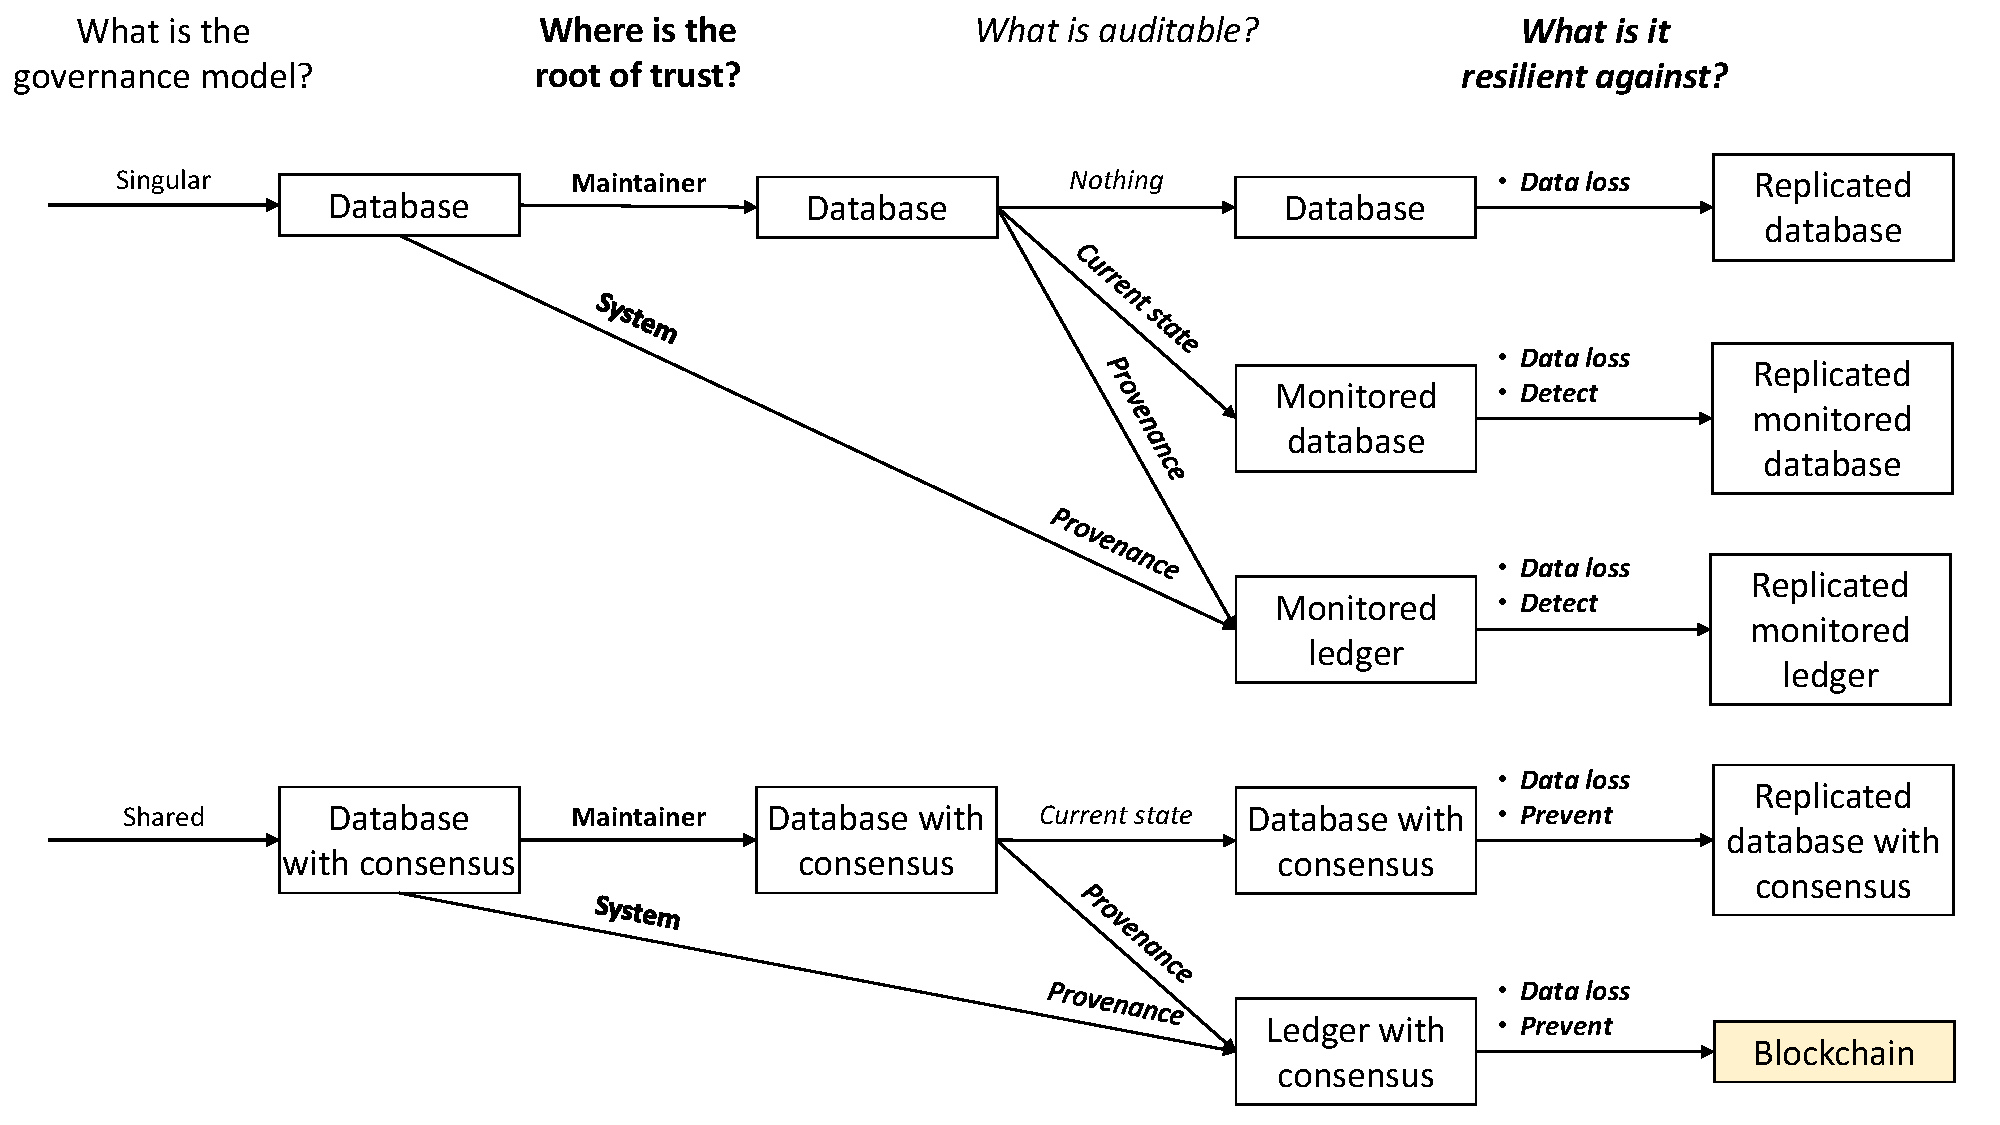
\includegraphics[width=\textwidth]{figures/BlockchainFlowchart}
	\caption{Comparing different distributed systems. Blockchain is highlighted in the bottom right corner.}
	\label{fig:blockchainFlowchart}
\end{figure*}

The first question is about who has the authority to manage and update the database: \emph{what is the governance model?} In a centrally governed database (a), a single entity performs these tasks. Alternatively, the system can use a consensus protocol such as Byzantine Agreement to allow for decentralized governance (b).

Next, we consider the security model by asking \emph{where is the root of trust?} This refers to the entity or entities that must behave honestly in order for the system to be secure. In typical database systems, trust is rooted in the maintainer -- for example, using AWS cloud storage requires that you trust Amazon. Alternatively, trust can be rooted in the design of the system itself. This is only possible if the system stores the provenance, or history, of the data in a verifiable way (e.g., as a hash chain or other authenticated data structure). Then auditors can confirm that data has not been manipulated by the maintainer or someone else. If this system is governed centrally, it is a monitored ledger (d), a good example of which is Google's Certificate Transparency project~\cite{CT}. If the system is decentralized, it is a historical ledger with consensus (f), where auditors can affirm that all changes to the data were made with valid consensus. To our knowledge, no such system exists, but it could be useful in some settings, such as publicly auditable committee votes. 

The next question is \emph{what is auditable?} If the system does not provide verifiable provenance, it can at least allow for verification of the current state. A simple way to do this is to publish a digitally signed hash of the full data store after each change. After each update, auditors will be able to verify that it was made by an authorized entity (the maintainer or the consensus group), but they cannot verify that the data has only been modified by authorized entities since its inception or that consensus has always been obeyed. Some software distribution repositories work this way, publishing a signed hash or checksum along with code updates. This system can be a centralized monitored database (c) or be run by decentralized consensus (e)\footnote{
	We omit the possibility of a consensus-based data store with no auditability because in a decentralized system, at a minimum consensus partners must be able to verify that state changes are made by consensus or the system cannot be trusted at all.
}. 

Finally, a database can have resilience properties depending on its design, so we ask \emph{what is it resilient against?} To prevent accidental data loss (e.g., by disk corruption), data can be replicated across multiple storage locations. A replicated database (g) is the simplest such system, but without current state auditing or verifiable provenance, malicious modifications cannot be detected or recovered from. If the system allows auditing (h, i), it can detect modifications, but auditors cannot recover lost or modified data. 

There are additional resilience properties that replicated storage can provide to a data store that is governed by a decentralized group. A replicated, monitored database with consensus (j) can recover from malicious updates as any changes not made by consensus will be rejected by replicating peers. The peer whose data was compromised will be overruled by the majority of honest peers. If the system also stores provenance so that the full history of changes can be verified back to the origin (even by users who join the system after its genesis), it is a full blockchain (k).

\subsection{Discussion}

\subsubsection{Is Blockchain a Good Fit for My Project?}

\subsection{Private Governance}
In our survey of the industrial literature, we encountered several systems that claimed to be Blockchain systems, but which did not have shared governance.
These systems resembled Blockchain systems, but with one critical difference: all the miners were controlled by a single entity.
The most prominent example of a private governance system is IBM's HyperLedger Fabric.
Interestingly, the HyperLedger Fabric software project allows for consortium governance, but IBM's implementation has IBM manage all of the miners.

Ultimately, we do not classify such systems as a part of Blockchain technology.
First, these systems do not have shared governance, which we identify as the key component of Blockchain technology.
Second, the party governing the system still represents a single-point of failure.
While the miners within the operating organization might be run on a distributed infrastructure, there is still a high chance that a sufficient compromise in the operating organization would lead to a compromise in the Blockchain system.
Third, there is nothing that prevents the governing party from deleting or modifying data; even if such changes could be detected, the data itself is not replicated outside the organization and would be lost.
Finally, most of the private governance are overly complex for what they are trying to accomplish.
Without the need for shared governance, many of these systems could be better implemented as a replicated monitored database.

\subsubsection{Off-Chain Oracles}
Several Blockchains systems need to access off-chain information during normal processing---for example, retrieving data from a Web site or ascertaining the result of a real-world event.
To do so, these systems rely on \emph{off-chain oracles} which are responsible for gathering external information and then recording that information within a transaction, making it available to the Blockchain system.
While such oracles are helpful, they do impact the the auditability of the system as it may not be possible to verify the off-chain oracle's answer at a later date.
As such, if such oracles are they introduce a trusted third-party into a system which otherwise relies on defused trust.
To address this issues, it is possible for off-chain oracles to be collectively operated by the miners.





\paragraph{Normative and technical properties are cleanly separable}
When reading papers or participating in discussions about Blockchain, it can be difficult to separate normative statements from technical ones (see section~\ref{subsec:challenges} for a discussion of this challenge). In our concept graph, however, technical properties and normative properties cleanly separate. No capabilities have dependencies on normative properties, and removing them from graph does not lessen the value of the graph as an exploration of technical concepts. The injection of ideology into a technical field causes confusion and suboptimal design choices -- not to mention muddying discussion and preventing clarity -- so we believe this surprising result is of value to the field in so far as it may help to resolve these issues.

\subsubsection{Anonymity and privacy are orthogonal to the core functions of a blockchain}
Several authors in our corpus cite \capability{anonymity} or privacy as features of Blockchain, although these terms are rarely defined precisely. The main belief seems to be that Blockchain has the property of \techproperty{anonymous transactions} -- i.e., it hides the sender and receiver of asset transfers and disassociates on-chain identities from real-world identities. These notions are connected to Blockchain's reputation for enabling illicit activity (see section~\ref{subsec:challenges} for a discussion of this challenge). The thinking goes that because Bitcoin is the currency of choice for illicit online purchases, it must be "untraceable", and as the most prominent blockchain-based system, distinctions are not drawn between properties of Bitcoin and properties of Blockchain.

Copious literature demonstrating the lack of privacy and anonymity in Bitcoin aside (\cite{Goldfeder17}, \cite{Conti17}, \cite{Androulaki13}, and others), our graph reveals that anonymity is a weakly-connected capability, leveraging few of Blockchain's core primitives and and supporting \textbf{no} use cases. While advanced cryptography like \primitive{multi-party computation}, \primitive{functional encryption}, and \primitive{zero-knowledge proofs} could be layered on top of a blockchain to provide some form of anonymity, only the last primitive appeared in our corpus. \techproperty{Key-based ownership of tokens} is the only property that supports anonymity and also derives from at least one core blockchain primitive (specifically, \primitive{authentication}).

\paragraph{Blockchain can serve as both a ledger and a data store, but it's better as a ledger}
Two highly-connected, central nodes in our graph are \techproperty{distributed data store} and \techproperty{distributed ledger}. Both rely on a \techproperty{consensus protocol} to ensure consistency across the different data storage locations. The distributed ledger further requires an \techproperty{append-only transaction ledger} to ensure that once consensus has been reached on a transaction, it can no longer be modified. 

As a distributed data store, Blockchain can provide two useful capabilities: \capability{data discovery} and \capability{resilience} (through \techproperty{replication}). As a distributed ledger, Blockchain also provides resilience through \capability{verifiable data store rebuilding} (which allows a node to recover to the current ledger state even if it suffers local data loss). Further, the ledger enables two important groups capabilities that support many use cases: \capability{auditability} and \capability{provenance}. 

This shows that Blockchain's significant novel utility is more firmly rooted in its ability to provide a distributed ledger of state changes than the simple maintenance of a single shared state.




\subsection{Challenges and limitations}
\label{subsec:challenges}

% Jeremy: I reclustered this a bit. I think we discussed this during the call. Feel free to debate. 
% If you want to play around with the clusters: https://drive.google.com/file/d/1gDVd4x-SN6-QHZe52toEzMWXnLfiNtqW/view?usp=sharing
% I feel like separating challenges and limitations is a bit of a judgement call. 

Our concept map shows interconnections between features and use cases. We also coded challenges -- both problems hindering the use of Blockchain that do not currently have satisfactory solutions, and inherent deficits of the technology. In this section, we will list the concept groupings we created and we discuss the academic response in the next section.
\anote{I really like this list.  But, the challenges in Section~\ref{sec:challenges} only cover a subset of the list (and its not divided in the same way).  Should we aim to cover all the challenges listed here (for many of them, I dont really know what to say)?  We should definitely get the two sections to match up better.}
\subsubsection{Technical Challenges}
\begin{itemize}
	\item{Blockchain can handle finite, countable, and unique resources only}
	\item{Blockchain is not a high performance system}
	\item{Lack of API access means auditors must run full nodes}
	\item{Interoperability: cryptocurrency fragmentation; existence of too many implementations; siloed solutions; standardization; risks to overlay assets if underlying assets are mishandled; interfaces with existing institutions and systems; user identification across systems; risks posed by sharing blockchain security through merged mining or anchoring}	
        \item{Susceptibility to coordinated attacks by large parties}
	\item{Off-chain functionality: off-chain program execution; interoperability with off-chain systems}
	\item{Privacy: anonymity; confidentiality}
	\item{Resilience: distributed denial-of-service (DDOS) attacks; dishonest majority attacks; security of infrastructure; subversion of software security measures}		
	\item{Scalability: block generation frequency; block size limits; computational cost of public blockchains; scalable and secure end-user software}
	\item{Security}
	\item{Smart contract correctness: inherent incompleteness of contracts; ensuring completeness; lack of tools for verification}
\end{itemize}

\subsubsection{Socio-Technical Challenges}
\begin{itemize}
	\item{Blockchain is an inefficient use of computing resources}
	\item{Cryptocurrency economics: illiquidity, price volatility, high initial adoption costs, currency conversion costs, and decreasing marginal returns for miners}
	\item{Incentives: correctly configuring game-theoretic incentive structures}
	\item{Key management: difficulty of manual key management; possible unrecoverable loss of private keys; attacks against wallets; bugs and glitches in wallets}	
	\item{Lack of protection against mistakes: transactions cannot be reversed; administrators cannot restore access if users are locked out}
	\item{Miner centralization}
	\item{Usability: difficulty of developing distributed apps; inherent complexity of technology; difficulty of access and use by consumers; education; onboarding users; difficulty of search; poor UX; lack of mobile and web clients}
\end{itemize}

\subsubsection{Challenges to Market Viability}
\begin{itemize}
	\item{Efficiency and cost: low or bottlenecked throughput; wasteful energy consumption; high transaction fees; latency induced by synchronous communication required by certain consensus protocols}
	\item{Expense of developing end-user applications for individual blockchains}
	\item{Usefulness: few demonstrable use cases; does not improve upon existing solutions in many domains being pursued}
	\item{Unnecessary: if a central party is required; if a trusted intermediary exists; if a small number of parties are involved in the system}
\end{itemize}

\subsubsection{Use Case Challenges}
\begin{itemize}
	\item{Binding digital entities to real-world entities: stapling tokens to assets; interoperating with existing systems (e.g., compatibility between cryptocurrencies and cash)}
	\item{Dispute resolution: difficulty recovering from errors or bugs; difficulty reversing fraudulent transactions; non-applicability to scenarios where a central broker is needed}
\end{itemize}

\subsubsection{Regulatory Challenges}
\begin{itemize}
	\item{Governance: resolution of conflicts requiring external intervention; incident response; rule updates require forks; transparency of software development}
	\item{No distinct legal framework}
	\item{Standardization}
	\item{Regulatory: anti-money laundering, know-your-customer; difficulty of monitoring; lack of regulation; legal considerations; taxation; exchange control and flow management; consumer protection}	
	\item{Cryptocurrencies are inherently Ponzi schemes}
	\item{Reputation: use for crime; associations with black markets; nebulous or illicit uses; terrorist financing}
\end{itemize}